\documentclass{hhu-thesis-bachelor}
%% 更改数学字体设置,Latin Modern Math 默认的有点细,可选用下列宏包
% \usepackage[bold-style=ISO]{unicode-math}
\usepackage{lipsum}

%% 本科论文规定不允许有空页,因此将空页替换掉
\let\cleardoublepage\clearpage

\begin{document}

%%
%% 基本信息设定(一定要改这里)
%%

% 此处填写你的学号
\studentnumber{2xxxxxxxxxxx}
% 此处填写你的中文论文标题
\title{论文名}
% 此处填写你的中文姓名
\author{xxx}
% 此处填写你的年级,如:2021级
\grade{2021级}
% 此处填写指导教师的中文名
\tutor{xxx}
% 此处填写专业的中文名
\major{xxxxxxx}
% 此处填写评阅人(答辩完成后填写,答辩时空着)
\reviewer{}
% 此处填写日期,如:2025年5月
\thesisdate{2025年5月}
% 此处填写中文地点,如:中~~国~~$\cdot$~~南~~京,将城市名改成所在的城市即可
\location{中国\enspace 南京}

% 此处填写英文论文标题
\englishtitle{xxxxxxxxxx}
% 此处填写英文学院名
\englishcollege{xxxxxxxxxxx}
% 此处填写英文专业名
\englishmajor{xxxxxxxxxx}
% 此处填写你的英文姓名
\englishauthor{xxxxxxx}
% 此处填写指导教师的英文名,教授使用 Professor,副教授使用 Associate Professor
\englishtutor{xxxx Associate Professor}
% 此处填写英文地点
\englishlocate{NANJING CHINA}

%% 填写完上述信息后,即可在chapters文件夹中创建tex文件开始写作,
%% 引用的参考文献以bib文件形式放在reference文件夹中,
%% 写作完成后,在下面的正文部分引入所有的tex文件,
%% 并在下面的参考文献部分引入所有bib文件,编译即可生成论文。

%%
%% 生成封面和声明页
%%

%% 生成中文封面
\makecover
%% 生成英文封面
\makeencover
%% 生成声明页
\makedeclare

%%
%% 前置部分
%%

\frontmatter
\pagestyle{hhuformatestyle}
%% 摘要
%% This is file 'abstract.tex'

\begin{abstract}
	\linespread{1.5}
由于泥沙与水流的相互作用,使得河流发生演变,因此泥沙特性与水流特性均是河流动力学的重要研究课题。当水流中含有植物时,水流的紊动特性会发生明显的改变,从而引起泥沙的一些特性如沉速发生改变。本文以实验为基础,结合理论分析,研究了在静水条件下刚性植物对泥沙沉速的影响,同时在水槽中通过改变流量来研究在恒定均匀流条件下非淹没植物对泥沙沉降轨迹的影响,得到如下主要结论:

此处填写中文摘要

% 中文关键词使用中文;隔开
\keywords{关键词1;关键词2;关键词3}
\end{abstract}


\begin{enabstract}
	\linespread{1.5}
Fluvial river processes evolve over time in response to the constant interaction between sediment and the water column. If vegetation is present within the water column, the change in turbulence characteristics will impact the movement of sediment, in particular the settling velocity. In this paper, the influence of vegetation on the settling velocities of sediment particles is studied experimentally. The  non-submerged vegetation friction factor in steady uniform flow is considered by under different flume discharge quantities. The main outcomes can be summarized as follows:

此处填写英文摘要

% 英文关键词使用英文;隔开
\enkeywords{sediment; rigid vegetation; settling velocity; turbulence characterize}

\end{enabstract}

%% 符号对照表,可选,如不用可注释掉
% \input{chapters/denotation}
%% 加入目录
\tableofcontents

%%
%% 正文部分(在这里引入你的所有tex文件和bib文件)
%%

\mainmatter

%% 各章正文内容
%% 在这里引入各章节,一般本科毕设五章,一章绪论+三章研究内容+一章总结展望
%% This is file 'chapter1.tex'

\chapter{绪论}
\label{chap:introduction}
\section{研究背景}
\label{sec:meaning}

当前,全球能源日益稀缺和环境污染问题持续加剧……

……

……2022年到2023年全国新能源汽车销量如图\ref{fig:xnll}所示:

\begin{figure}[H]
    \centering
    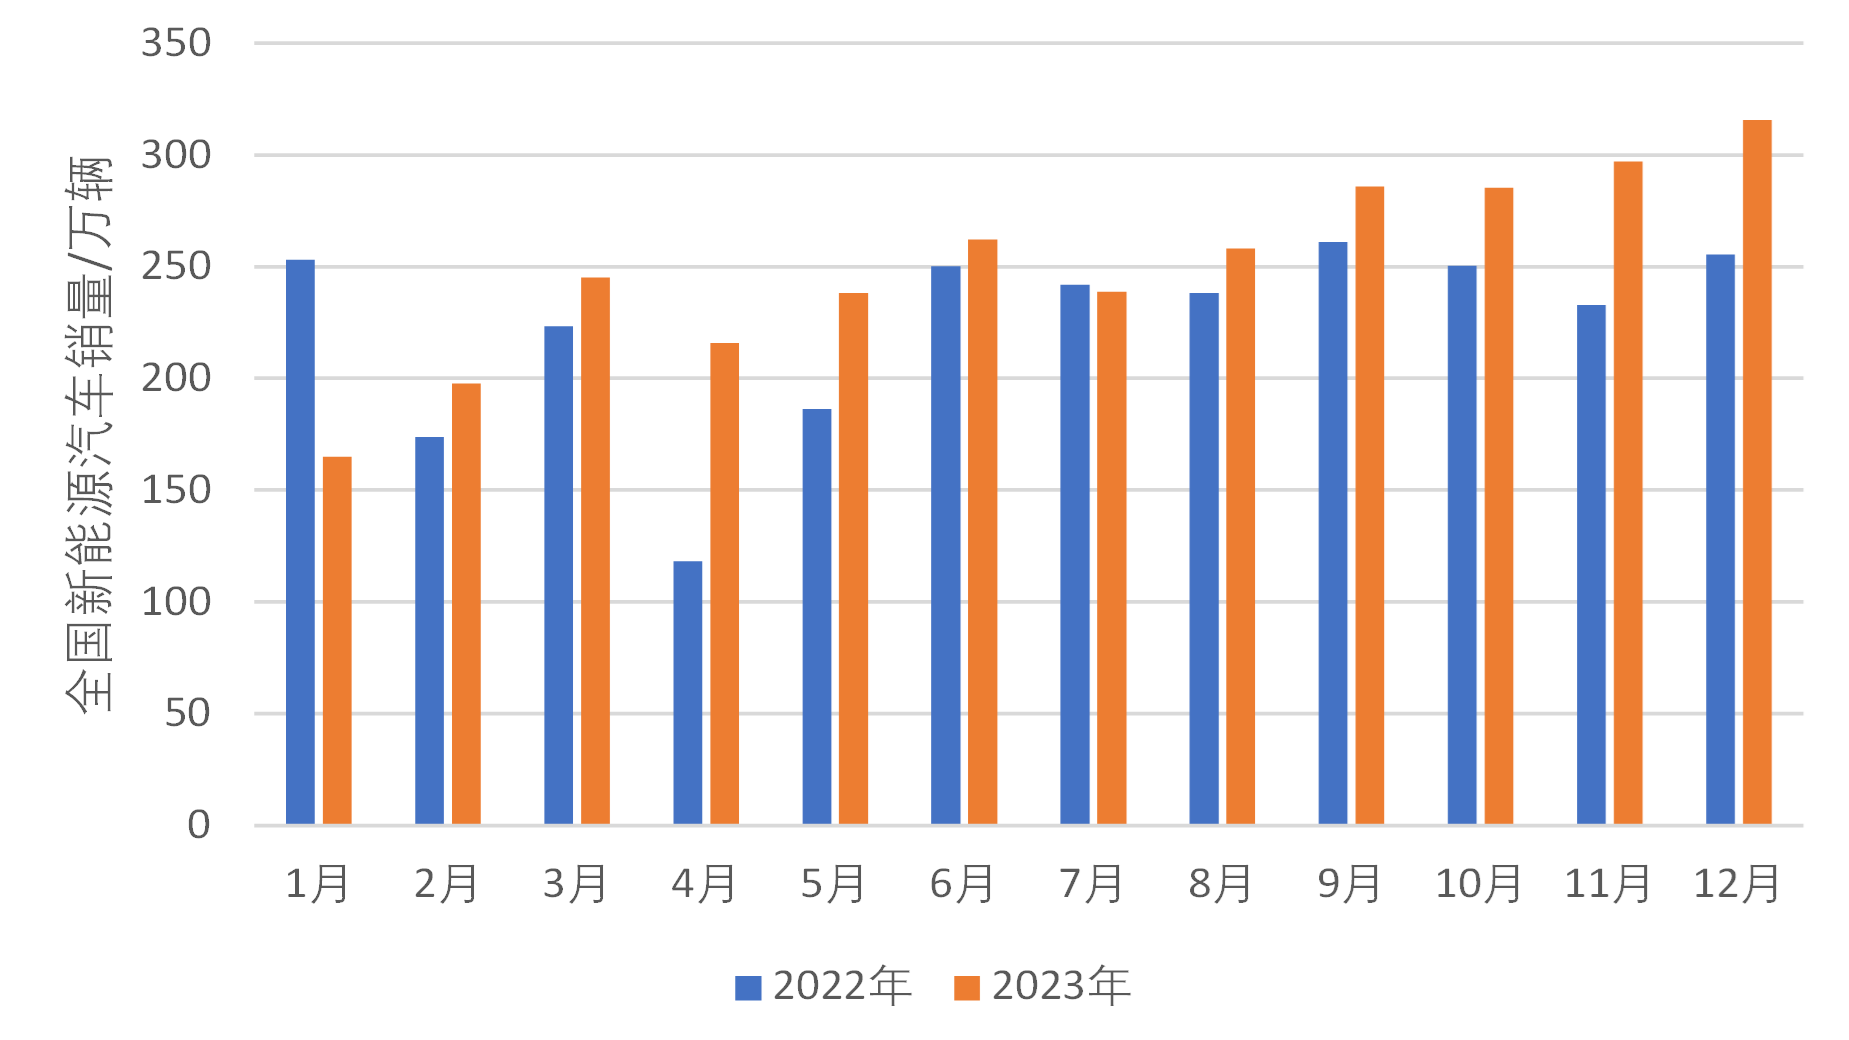
\includegraphics[width=0.9\textwidth]{figures/xnll.png}
    \caption{全国新能源汽车销量}
    \label{fig:xnll}
\end{figure}

虽然电动汽车的大规模应用一定程度上减轻了能源危机和环境恶化,但电动汽车作为具有源负荷性质的柔性负载\upcite{buzna2021ensemble}……

\section{国内外研究现状}

\subsection{xxxx研究现状}

电动汽车成为研究热点以来,国内外学者对电动汽车充电负荷进行了广泛的研究,目前主要集中从电动汽车(Electric Vehicles, EV)时间特性上整体建模。文献\cite{1021704678.nh}……

\section{本文主要工作}

%% This is file 'chapter2.tex'

\chapter{基于蒙特卡洛的}
\label{chap:inverseproblem}

\section{引言}
引言……

……

\section{xxxxxxx影响因素分析}

\subsection{xxx细分}

……概率密度函数为:
\begin{equation}
\label{eq:kduiuijm}
    f_s(t_1)=\left\{
    \begin{array}{lr}
    \frac{1}{\sigma_s\sqrt{2\pi}}e^{-\frac{(t_1-\mu_s)^2}{2\sigma_s^2}}, & \mu_S-12<t_1\leq 24\\
    \frac{1}{\sigma_s\sqrt{2\pi}}e^{-\frac{(t_1+24-\mu_s)^2}{2\sigma_s^2}}, & 0<t_1\leq \mu_s-12
    \end{array}
    \right.
\end{equation}
\noindent 式中:$t_1$为开始充电时间;$\mu_S$为函数$f_s(t_1)$中$t_1$的期望;$\sigma_S$为$f_s(t_1)$中$t_1$的标准差。

……如表\ref{tab:parameter}和表\ref{tab:gdlv}所示:

\begin{table}[H]\small
    \centering
    \caption{不同类型电动汽车日行驶里程对数正态分布参数}
    \label{tab:parameter}
    \begin{tabularx}{\textwidth}{@{} >{\centering\arraybackslash}X >{\centering\arraybackslash}X >{\centering\arraybackslash}X >{\centering\arraybackslash}X @{}}
    \toprule
	参数 & 私家车 & 公交车 & 出租车\\\midrule
    $\mu_D$ & 3.2 & 3.0 & 5.1\\
    $\sigma_D$ & 0.88 & 0.8 & 0.3\\
    \bottomrule
    \end{tabularx}%
\end{table}

\begin{table}[H]\small
    \centering
    \caption{不同电动汽车开始充电时间和概率}
    \label{tab:gdlv}
    \begin{tabularx}{\textwidth}{@{} >{\centering\arraybackslash}X >{\centering\arraybackslash}X >{\centering\arraybackslash}X >{\centering\arraybackslash}X \>{\centering\arraybackslash}X @{}}
    \toprule
	{电动汽车类型 & 功能区 & 充电时段 & 充电概率 & 充电开始时间分布}\\\midrule
    \multirow{2}{*}{出租车} & \multirow{2}{*}{商业区} & 02:00$\sim$04:00 & 100\% & \multirow{2}{*}{均匀分布}\\
    \cline{3-4}
    & & 11:30$\sim$4:00 & 100\% &\\\midrule
    公交车 & 工作区 & 18:00$\sim$08:00 & 100\% & 均匀分布\\\midrule \multirow{2}{*}{私家车} & 工作区 & 08:00$\sim$17:00 & 20\% & $N(8.9,1.5^2)$\\\cline{2-5}
    & 居民区 & 17:00$\sim$07:00 & 80\% & $N(17.6,3.4^2)$\\
    \bottomrule
    \end{tabularx}
\end{table}


\section{本章小结}

\chapter{xxxx}

\section{引言}

\section{xxxxx}


\chapter{xxxxxxxxxxxxxxxxx}


\chapter{总结与展望}

\section{总结}


\section{展望}


%% (其后部分无编号)
\backmatter
%% 引入致谢
%% This is file 'acknowledgement.tex'

\begin{acknowledgement}

此处编写感谢

\vspace{5cm}
\begin{flushright}
	作者:xxxx\\
	2024年5月于南京
\end{flushright}

\end{acknowledgement}

%% 参考文献样式设定
\bibliographystyle{hhuthesis-numeric}% 顺序编码式

%% 参考文献,10号字,使用 BibTeX,包含参考文献文件.bib
%% 如果新创建了bib文件,记得要在这里引用哦!!!
\bibliography{reference/chap1}

\end{document}